\documentclass[serif]{beamer}

\newcommand{\LE}{\emph{Let's Encrypt~}}%
\newcommand{\LEs}{\emph{Let's Encrypt}}%
\usenavigationsymbolstemplate{}
\addtobeamertemplate{navigation symbols}{}{%
    \usebeamerfont{footline}%
    \usebeamercolor[fg]{footline}%
    \hspace{1em}%
    \insertframenumber/\inserttotalframenumber
}


\usepackage{hyperref}
\usepackage{cancel}

\hypersetup{
    colorlinks,%
    citecolor=red,%\ne
    filecolor=black,%
    linkcolor=blue,%
    urlcolor=red
}

\setbeamerfont{footline}{series=\bfseries, size=\footnotesize}

\title{Anomaly Detection on DNS Auths }
\subtitle{Root DNS, ccTLDs and DNS providers}

\author[\large \textbf{Team \cancel{Schnabeltier}}

]
{\large \textbf{Team \cancel{Schabeltier}Anomalizers}\\
\vspace{0.5cm}
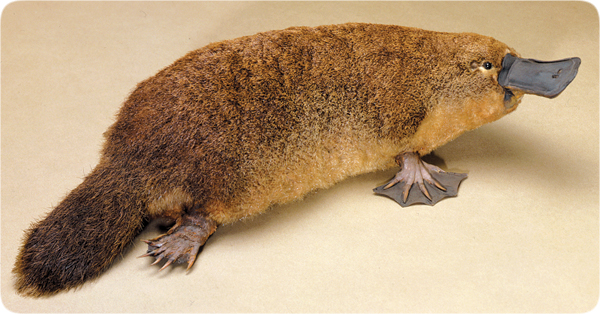
\includegraphics[width=5cm]{fig/Schnabeltier.jpg}
}

\date[IETF98] % (optional)
{RIPE DNS Hackaton 2017\\Amsterdam, The Netherlands\\
2017-04-21}

% \logo{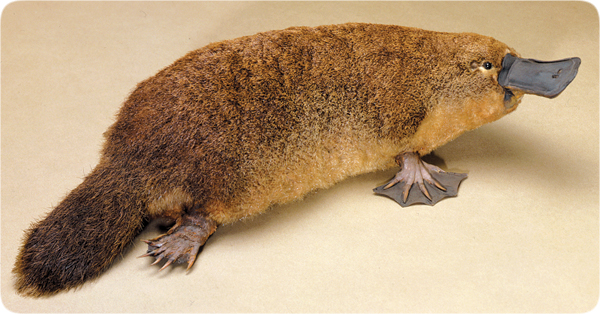
\includegraphics[scale=0.051]{fig/Schnabeltier.jpg}}

\begin{document}
\frame{\titlepage}

\section{At a glance}

\begin{frame}
	\frametitle{Team Members (alphabetically)}
	
	\begin{itemize}
	\item Christian Doerr (TU Delft)
	\item Ella 
	\item Giovane Moura (SIDN Labs)
	\item Jan Harm Kuipers (University of Twente/SIDN Labs)
	\item Moritz M\"uller (SIDN Labs/University of Twente)
	\item Ricardo Schmidt (University of Twente)
	\item Wouter de Vries (University of Twente)
% 	\item 
	\end{itemize}


\end{frame}

\begin{frame}
	\frametitle{Resources}
	
	\begin{itemize}
	  \item GitHub: \url{https://github.com/orgs/ripe-dns-anomaly/}
	  \item Demo: \url{https://ripe-dns-anomaly.github.io}
	\end{itemize}


\end{frame}



\begin{frame}
	\frametitle{Main Problem}
	
	\begin{block}{Auth DNS Anomaly Detection}
	\begin{itemize}
	 \item \textit{How can we use Ripe Atlas data to detect automatically 
failures on Auth DNS (Roots, ccTLDs, etc...)?}
	\end{itemize}

	\end{block}

\end{frame}


\begin{frame}[fragile]
	\frametitle{Step-by-step - CHAOS/RTT}
	
\begin{enumerate}
 \item Download Ripe datasets and parse them
 \begin{itemize}
  \item \url{https://github.com/ripe-dns-anomaly/chaos }
  \item \texttt{parse-json.sh \$startTime \$endTime bins}
  \item start and end = timestamps
  \item bins= 600 (10minutes)
 \end{itemize}

 \item Then, run anomaly detection per letter and site:
 \begin{itemize}
  \item \url{https://github.com/ripe-dns-anomaly/anomalyDetector}
  \item \texttt{python letter-level-detector.py data/k-root-ddos-20151130.csv 
output/k-root-ddos-20151130-ad-hoc.csv}
 \end{itemize}

\item Then, it outputs anomalies per class type:
\begin{itemize}
 \item 
\url{https://github.com/ripe-dns-anomaly/anomalyDetector/blob/master/README.md}
\end{itemize}

\end{enumerate}


\end{frame}

\begin{frame}[fragile]
	\frametitle{Step-by-step - Path}
	
\begin{enumerate}
 \item Download Ripe datasets and parse them
 \begin{itemize}
  \item \url{https://github.com/ripe-dns-anomaly/traceroute }
  \item \texttt{python traceget.py --start \$startTime --end \$endTime --msmid \$msmid}
  \item start and end = timestamps
  \item msmid = atlas measurement id (5001 for K-root)
 \end{itemize}

 \item Then, convert the format:
 \begin{itemize}
  \item \url{https://github.com/ripe-dns-anomaly/traceroute}
  \item \texttt{java -jar}
 \end{itemize}

 \item Last step: convert to webformat
\end{enumerate}

\end{frame}

\begin{frame}[fragile]
	\frametitle{Algorithms for Anomaly Detection}
	\begin{itemize}
	 \item See discussion on 
\url{https://github.com/ripe-dns-anomaly/anomalyDetector/blob/master/README.md}
	\item Twitter's robust TS analysis, ARIMA, ad-hoc
	\item We choose ad-hoc (ours)
	\item Data is not periodical
	\item We need more time to evaluate the best one
	\item Less false positives
	\end{itemize}


\end{frame}


\begin{frame}[fragile]
	\frametitle{Demo}
	
	\large
	\url{https://ripe-dns-anomaly.github.io}

\end{frame}


\begin{frame}[fragile]
	\frametitle{Ready to be used by others}
\begin{itemize}
 \item Use by ccTLDs, Roots, etc.
 \item Requirement: Ripe Atlas measurements with \textbf{chaos.id} support
 \item Next: automate it to continuously probe it, detect and notify
\end{itemize}

\end{frame}


\end{document}
